\documentclass{article}

\usepackage{booktabs}
\usepackage{multirow}
\usepackage{amsmath}
\usepackage{hyperref}
\usepackage{overpic}
\usepackage{amssymb}

\usepackage[accepted]{dlaiml2026}

\usepackage{todonotes}[inline]

\dlaititlerunning{SQ-DiT: SliderQuant for Diffusion Models}

\begin{document}

\twocolumn[
\dlaititle{SQ-DiT: SliderQuant for Diffusion Models}

\begin{center}\today\end{center}

\begin{dlaiauthorlist}
\dlaiauthor{Simone Lidonnici - 2061343}{}
\dlaiauthor{Pietro Adamo Morelli - 2087359}{}
\end{dlaiauthorlist}

\dlaicorrespondingauthor{\newline Simone Lidonnici}{lidonnici.2061343@studenti.uniroma1.it}
\dlaicorrespondingauthor{\newline Pietro Adamo Morelli}{morelli.2087359@studenti.uniroma1.it}

\vskip 0.3in
]

\printAffiliationsAndNotice{}

\begin{abstract}
Diffusion Transformers (DiTs) have recently established a new baseline for image generation models, but their major limitations are the heavy computational and memory requirements.
To mitigate these bottlenecks, Post-Training Quantization (PTQ) offers a practical approach to compress these models without retraining.
In this project, we adapt SliderQuant, a PTQ algorithm originally designed for Large Language Models (LLMs), to the visual generation domain.
Code is available at: \url{https://github.com/DoctorWho28/deepLearning}.
\end{abstract}


\section{Introduction}\label{sec:intro}

Diffusion Transformers (DiT) created a new standard of generative AI, replacing the convolutional U-Net backbone of diffusion models with a Transformer architecture.
DiTs rely on \textbf{Adaptive Layer Normalization (AdaLN)} to inject continuous timestep and discrete class conditionings into each block, dynamically adapting intermediate feature states at each denoising step.
DiTs achieve remarkable results in high-fidelity image generation, but their large parameter count and iterative approach lead to prohibitive memory consumption (VRAM) and slow inference speeds.
To mitigate these computational bottlenecks, Post-Training Quantization (PTQ) techniques compress the weights to lower-bit formats without requiring a full model retraining.


Recently, a PTQ framework named \textbf{SliderQuant} was introduced for Large Language Models (LLMs).
SliderQuant exploits the fact that different layers in deep networks have different sensitivities to quantization noise. It introduces a sliding-window distillation approach, optimizing quantization parameters over small groups of layers, and introduces learnable low-rank matrices (LoRA) to compensate for the quantization error.

SQ-DiT aims to adapt the core concepts of SliderQuant to Diffusion Transformers.
The main difference is that SliderQuant calibrates LLMs over sequential tokens, whereas DiTs require optimizing across the temporal diffusion process.
During the optimization process, the weights are quantized using fake quantization and only upon completion the final weights are packed into INT8 using our custom packing implementation to effectively save VRAM space.
\todo{Aggiungere la specificazione sui modelli ImageNet-1k class-to-image e scrivere del modello \href{https://huggingface.co/facebook/DiT-XL-2-256}{facebook/DiT-XL-2-256}}


\section{Related works}\label{sec:related}

SQ-DiT derives from SliderQuant \cite{wang2026sliderquantaccurateposttrainingquantization} adapting the quantization and distillation concepts to the DiT architecture.

PTQ4DiT \cite{wu2024ptq4ditposttrainingquantizationdiffusion} and Q-DiT \cite{chen2024qditaccurateposttrainingquantization} serve as our primary foundational references for the state of the art in PTQ for DiTs.

\todo{Possibile escursus sui paper usati per confrontare i risultati}


\section{Method}\label{sec:quant}

\subsection{SliderQuant}

SliderQuant builds on the premise that initial (shallow) and terminal (deep) layers have higher quantization sensitivity than intermediate ones.
These boundary layers are optimized using a progressively expanding window, while the intermediate layers are optimized using a fixed size sliding-window.
In both cases, layers in the same window are quantized jointly.

To minimize the weight quantization error, an optimizer is applied to a set of learnable parameter for each linear module, specifically a scaling factor ($\alpha$) and two low-rank LoRA matrices ($A$ and $B$).

To soften the impact on the weights and avoid eccessive parameter perturbations, quantization is performed in two progressive stages: a partial quantization is applied according to a ratio $\gamma$, followed by the full quantization.
To mitigate the impact of extreme weight values, we apply group-wise quantization, confining outliers to local groups and preserving the precision of the remaining parameters.


\subsection{SQ-DiT implementation}
Because the original SliderQuant framework cannot be easily transposed, we developed the entire quantization framework from scratch.
\todo{Scrivere della creazione della classe SliderQuantLinear e della funzione \texttt{forward()}}


\paragraph{Timestep-Aware Window Distillation.}

We group transformer blocks into sliding windows and optimize them sequentially.
For each window, we optimize the quantization parameters by minimizing the Mean Squared Error (MSE) between the output features of the quantized blocks with their original unquantized counterparts. SliderQuant uses the $L^2$ norm intead of the MSE.
\todo{Capire se scrivere meglio questa differenza}

Unlike LLMs, where the input passes through each block only once, in DiT models the image is gradually denoised across multiple timesteps, passing through all the blocks at each step.

Since data distributions change drastically throughout the denoising process, a quantization approach that propagates error across the timesteps would be unstable.
For this reason, rather than allowing the error to propagate over time, each window jointly optimizes multiple timesteps.
We provide the first block with the latents pre-calculated by the original FP16 model across all timesteps, while the subsequent blocks receive the output of the preceding quantized block.

By eliminating temporal propagation, we align the optimization with the SliderQuant paradigm used for LLMs, that don't have noise accumulation between timesteps.
This allows the LoRA matrices within each window to focus exclusively on compensating for spatial errors propagated by preceding quantized layers.

\todo{vedere se specificare che vengono fatte anche diverse classe congiuntamente}

\paragraph{Mixed-Precision Architecture.}

Following the original observation that network layers exhibit varying sensitivities to quantization, we decided to augment the SliderQuant approch by applying a mixed-precision policy.
Deep and shallow transformer blocks are highly sensitive and are therefore quantized to higher bit-widths (INT8 in our case) while intermediate layers, which are more robust to quantization noise, can be quantized to a lower bit-widths.

Other than that, crucial modules responsible for condition injection require special treatment. 
The initial \texttt{emb} module, which maps discrete time and class conditions into a continuous embedding space, is kept in FP16.
Since this conditioning guides the entire generative process, any error introduced here would cascade through all subsequent layers and degrade the feature representations.
Similarly, the AdaLN (\texttt{norm1}) module, responsible for injecting temporal and class features to the network, is quantized to higher precision. Aggressively quantizing this layer would cause the network to lose temporal awareness and class concepts, leading to generation failures.

Using this mixed-precision approach has a slight impact on VRAM utilization, but this is negligible compared to the benefits on generation stability.

\paragraph{Weights Packing.}

To effectively have an impact on the model size and VRAM utilization we implemented a custom \texttt{WXAXLinear} module as a replacement for standard linear layers.
This module physically packs low-bit quantized weights into \texttt{INT8} using bitwise shift and masking operations.
\todo{Spiegare come vengono fatti gli shift per INT4 e INT2}

When loading the model to generate an image, we replace the original linear layers with their \texttt{WXAXLinear} counterparts and load the packed weights into memory.
During inference, the layer performs on the fly unpacking, restoring the weights to FP16 dynamically to continue the image generation process.



\section{Evaluation}\label{sec:eval}


\begin{table}[h!]
    \caption{Evaluation comparison}
    \label{tab:evaluation}
    \centering
    \begin{small}
        \begin{tabular}{c|ccccc}
            \toprule
            &Size&FID $\downarrow$&IS $\uparrow$&sFID $\downarrow$&CMMD $\downarrow$\\
            \midrule
            FP16&1.58 GB&24.72&318 $\pm$ 7.9&59.3&0.236\\
            W8A8&0.97 GB&24.48&322 $\pm$ 6.0&57.8&0.239\\
            W4A8&0.78 GB&23.49&314 $\pm$ 6.7&55.7&0.236\\
            \bottomrule
        \end{tabular}
    \end{small}
\end{table}
\todo{Cambiare ordine in FID, sFID, IS, CMMD}

\begin{table}[h!]
    \caption{Delta comparison}
    \label{tab:delta}
    \centering
    \begin{small}
        \begin{tabular}{cc|ccccc}
            \toprule
            &Method&$\Delta$ size&$\Delta$FID&$\Delta$IS&$\Delta$sFID\\
            \midrule
            \multirow{3}{*}{W8A8}&PTQ4DiT&-1.9 GB&-0.5&4.44&-2.2\\
            &ViDiT&-75 \%&-8 \%&+1.8 \%&-11\%\\
            &Ours&12&56&78&45\\
            \midrule
            \multirow{3}{*}{W4A8}&PTQ4DiT&25&45&67&17\\
            &ViDiT&89&56&13&34\\
            &Ours&12&56&78&45\\
            \bottomrule
        \end{tabular}
    \end{small}
\end{table}


Si può vedere un esempio delle differenze per un'immagine nella figura \ref{fig:image_comparison}.


\begin{figure}[t]
    \centering
    \begin{minipage}[b]{0.32\linewidth}
        \centering
        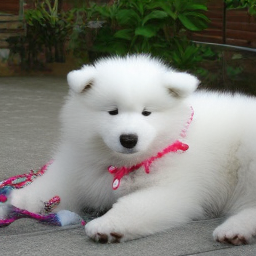
\includegraphics[width=\linewidth]{images/fp16_image.png}
        \centerline{\small (a) Original}
    \end{minipage}
    \hfill
    \begin{minipage}[b]{0.32\linewidth}
        \centering
        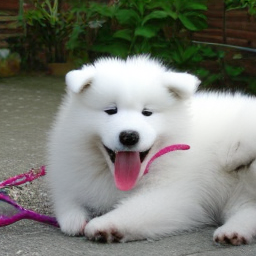
\includegraphics[width=\linewidth]{images/w8a8_image.png}
        \centerline{\small (b) W8A8}
    \end{minipage}
    \hfill
    \begin{minipage}[b]{0.32\linewidth}
        \centering
        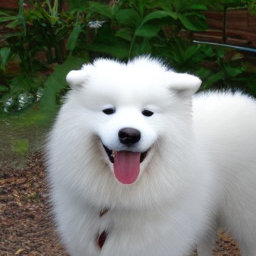
\includegraphics[width=\linewidth]{images/w4a8_image.png}
        \centerline{\small (c) W4A8}
    \end{minipage}
    \caption{Visual comparison of generated samples}
    \label{fig:image_comparison}
\end{figure}


\section{Conclusions}\label{sec:conc}





\cleardoublepage
\section*{Statement on the use of AI}\label{sec:ai}
%
Students must include a brief statement describing whether AI tools were used in the project and, if so, how they were used. This declaration is required for transparency, but it is not intended to penalize the use of AI in any way. A project may receive any grade in the full $0 - 31$ range regardless of whether AI tools were used extensively, minimally, or not at all.

The statement should clearly indicate the role of AI in the project. Examples include, but are not limited to: rephrasing or editing parts of the report, assisting with code writing, implementing core algorithms, preparing experiment scripts, debugging, data processing, literature exploration, or generating plots and other supporting material. Students are expected to be honest and sufficiently specific.

The responsibility for the submitted work always remains with the student(s). In particular, students must fully understand, verify, and be able to explain any material produced with the help of AI tools.

\textbf{Misuse of AI will be penalized.} Examples include submitting AI-generated material that the student does not understand, cannot justify, or cannot explain if required to do so; presenting AI-produced text, code, experimental results, or claims as if they had been independently developed or verified when this is not the case; or providing inaccurate or misleading declarations about the actual use of AI in the project.

There is no strict length limit for this section, but in most cases one column or less should be sufficient.

\bibliography{references.bib}
\bibliographystyle{dlaiml2026}

\section*{Appendix}

\paragraph{Adaptive Layer Normalization (AdaLN)}

\paragraph{Sensitivity analysis}

\paragraph{Simulation parameters}

\paragraph{Final weights formula}
\[W = W \cdot \alpha + A \times B\]

\end{document}

